\chapter{Introduction}\label{CH:introduction}
Above Earth's atmosphere are the Van Allen radiation belts, a complex and dynamic plasma environment that can effect our technology-driven society. These effects include: a higher radiation dose for astronauts and cosmonauts, higher chance of spacecraft failure due to single event upsets that can lead to catastrophic latchups, cumulative degradation of silicon (changing the silicon doping) from an extended radiation dose that can degrade a transition to the point where it no longer function as a switch, and the degradation of the ozone layer due to the chemical production of NOX and HOX. With these effects in mind, it is no surprise that the radiation belts have been extensively studied since their discovery in the 1960s.

A topic of interest in the space physics community is wave-particle intersections that as we will see later in the introduction, can accelerate particles and scatter them into the atmosphere.

The goal of this dissertation is to study the wave-particle mechanism that scatters microbursts into Earth's atmosphere. This goal will be achieved by first introducing single charged particle motion in electric and magnetic fields, the major particle populations and how they couple in the magnetosphere, and then describe the history and current state of the fields relating to microbursts and wave-particle scattering

\section{Charged Particle Motion in Electric and Magnetic Fields}\label{Intro:particle_motion}
A charged particle trapped in the magnetosphere will experience three types of periodic motion in Earth's nearly dipolar field. The three motions are ultimately due to the Lorentz force that a particle of momentum $\vec{p}$, charge $q$, and velocity $\vec{v}$ experiences in an electric field $\vec{E}$ and magnetic field $\vec{B}$ and is given by
\begin{equation}
\frac{d\vec{p}}{dt} = q(\vec{E} + \vec{v} \times \vec{B}).
\end{equation} In the magnetosphere, the three periodic motions in decreasing frequency are gyration, bounce, and drift and are schematically shown in Fig. \ref{Intro:motion_diagram}. Each of periodic these motions have a corresponding conserved quantity i.e. an adiabatic invariant. 

\begin{figure}
\includegraphics[width=\textwidth]{1_three_motions.png}
\caption{A diagram of the three motions that a charged particle experiences in Earth's dipole magnetic field. These motions are: gyration about the magnetic field line, bounce motion between the magnetic poles, and azimuthal drift around the Earth. Figure from \citep{Baumjohann1997}}
\label{Intro:motion_diagram}.
\end{figure}


The highest frequency periodic motion is on the order of a kHz in the magnetosphere and is gyration about a magnetic field of magnitude $B$. This motion is circular with a Larmor radius of 
\begin{equation}
r = \frac{m v_\perp}{|q| B}
\end{equation} where $m$ is the mass and $v_\perp$ the particle velocity perpendicular to $\vec{B}$. This motion has a corresponding gyrofrequency 
\begin{equation}
\Omega = \frac{|q| B}{m}
\end{equation} in units of radians/second. The corresponding adiabatic invariant can be found by integrating the particle's canonical momentum around the particle's path
\begin{equation}
J_i = \oint (\vec{p} + q \vec{A}) \cdot d\vec{l}
\end{equation} where $J_i$ is the $i^{th}$ adiabatic invariant and $\vec{A}$ is the magnetic vector potential. This integral is carried out by integrating the first term over the circumference of the gyro orbit and integrating the second term using Stokes theorem to calculate the magnetic flux enclosed by the gyro orbit.  With suitable integration, $J_1 \sim v_\perp^2 / B$ that is conserved as long as a driving force on the particle has a frequency much less than $\Omega$.

The second highest frequency periodic motion is the bounce motion that is due to a parallel gradient in $\vec{B}$. This periodic motion naturally arises in the magnetosphere because the Earth's magnetic field is stronger near the poles, and artificially in the laboratory in magnetic bottle machines. First we need to define the concept of pitch angle $\alpha$ as the angle between the magnetic field and particle's velocity vectors. This is schematically shown in Fig. \ref{Intro:pa}a. The pitch angle relates $v$ with $v_\perp$, and $v_{||}$ (the component of the particles velocity parallel to $\vec{B}$). As shown in \ref{Intro:pa}b and c, a larger $\alpha$ will tighten the particle's helix trajectory and vice versa.

Assuming that the particle's kinetic energy is concerned, the conservation of $J_1$ implies that given a particle's $v_\perp(0)$ and $B(0)$ at the magnetic equator, we can calculate its $v_\perp(s)$ along the particle's path with $B(s)$ from magnetic field models. The perpendicular velocity is related via
\begin{equation}
\frac{v_\perp^2 (0)}{B(0)} = \frac{v_\perp^2 (s)}{B(s)}
\end{equation} which can be rewritten as 

\begin{equation}
\frac{v^2 \sin^2{\alpha(0)}}{B(0)} = \frac{v^2 - v^2_{||}(s)}{B(s)}
\end{equation} and re-arranged to solve for $v_{||}(s)$

\begin{equation} \label{Intro:eq_vp} 
v_{||}(s) = v \sqrt{1 - \frac{B(s)}{B(0)} \sin^2{\alpha(0)}}
\end{equation} which will tend towards 0 since $B(s) > B(0)$ in a dipole magnetic field.

The location where $v_{||} = 0$ is called the mirror point where a particle stops and reverses direction. Since Earth's magnetic field is stronger towards the poles, the particle will execute periodic bounce motion between the two mirror points. The corresponding adiabatic invariant, $J_2$ is

\begin{equation} \label{Intro:j2}
J_2 = \oint p_{||} ds
\end{equation} where $ds$ describes the particle path between the mirror points in the northern and southern hemispheres. Substituting Eq. \ref{Intro:eq_vp} into Eq. \ref{Intro:j2} and using the fact that at the mirror point the magnetic field strength is $B_m$ and $\alpha(m) = 90$, $J_2$ can be written as     
\begin{equation}
J_2 = 2 p \int_{S \ mirror}^{N \ mirror} \sqrt{1 - \frac{B(s)}{B(m)}} ds
\end{equation} where $N \ mirror$ and $S \ mirror$ are the northern and southern mirror points, respectively. The bounce period can be estimated \citep[e.g.][]{Baumjohann1997} to be 

\begin{equation}
t_b \approx \frac{L R_e}{\sqrt{W/m}} (3.7 - 1.6 \sin{\alpha_0})
\end{equation} where $L$ is the $L$-shell which describes the distance from the Earth's center to where a particular magnetic field line crosses the magnetic equator, in units of Earth radii, $R_e$. $W$ is the particle's kinetic energy, and $\alpha_0$ is the equatorial pitch angle.

\begin{figure}
\includegraphics[scale=1]{1_pitch_angle_and_helix.png}
\caption{Charged particle motion in a uniform magnetic field $\vec{B}$. Panel (A) shows the geometry defining the pitch angle, $\alpha$. Panel (B) and (C) show two helical electron trajectories assuming a large and small $\alpha$ (corresponding to a small and large parallel velocity $v_{||}$), respectively.}
\label{Intro:pa}
\end{figure}

\textcolor{red}{In the presence of an electric field, $\vec{E}$, the particle will gyrate about its gyro center and the gyrocenter will drift due to the $\vec{E} \times \vec{B}$ drift.}

\section{Particle Populations and Their Interractions in the Magnetosphere}\label{ntro:particle_populations}

\section{Radiation Belts}\label{Intro:radiation_belt}
The Van Allen radiation belts were discovered by \citet{Allen1959} and \citet{Vernov1960} during the Cold War.

\subsection{Inner Magnetosphere Coordinates}\label{Intro:coords}


 No one had predicted the
existence of Earth’s radiation belts—
nested tori of energetic particles trapped
by the planet’s magnetic field

\subsection{Particle Acceleration}\label{Intro:acceleration}

\subsubsection{Adiabatic Heating}\label{Intro:adiabatic_heating}

\subsubsection{Wave Resonance Heating}\label{Intro:wave_heating}

\subsection{Particle Losses}\label{Intro:acceleration}

\subsubsection{Electromagnetic Ion Cyclotron Wave Driven}\label{Intro:emic_scattering}

\subsubsection{Whistler Mode Chorus Wave Driven}\label{Intro:chorus_scattering}

\section{Scope of Reserach}\label{Intro:scope}
This dissertation furthers our understanding of the microburst scattering mechanism and is organized into the following chapters. Chapter \textcolor{red}{X} will describe the spacecraft missions used to study microburst precipitation and wave-particle scattering. Then Ch. \textcolor{red}{Y} will describe a microburst scattering event observed by NASA's Van Allen Probes and the quasi-linear diffusion model that was developed. Next, Ch. \textcolor{red}{Z} will describe a bouncing packet microburst observation made by MSU's FIREBIRD-II mission where the microburst's lower bound longitudinal and latitudinal scale sizes were estimated. Chapter \textcolor{red}{ZZ} then expands the case study result from Ch. \textcolor{red}{Z} to a statistical study of microburst sizes and the microburst size models developed to interpret the data. Lastly, \textcolor{red}{ZZZ} will summarize the dissertation work and make concluding remarks about research to be done.

\iffalse %%%%%%%%%%%%%%%%%%%%% TEMPLATE %%%%%%%%%%%%%%%%%%%%%%%%%%%%%%%%%%%%
Welcome to the Montana State University electronic Thesis/Dissertation (ETD) \LaTeX{} template.  In this chapter various sections, subsections, and subsubsections are created and filled with random text).  In Ch.~\ref{CH:theory} methods to write equations and how to include figures and tables are explored. Conclusions are drawn in Ch.~\ref{conclusion}.


\section{Section}\label{Sect:test}
\lipsum[1] % Random text

\subsection{Subsection}\label{Sect:testsub}
\lipsum[2] % Random text

\subsubsection{Subsubsection}\label{Sect:testsubsub}
\lipsum[3] % Random text

\longsubsection{Subsection With a Very Very Very Very}{Very Very Very Very Very Very Long Title}\label{Sect:longsub}
For long subsection titles use the command \verb|\longsubsection{#1}{#2}|, where \#1 is the first line of the long title, and \#2 is the second line of the long title. You can also pass an optional argument to this command that puts a shorter title in the table of contents as shown by the subsection below.

\longsubsection[Subsection With a Very Long Title]{Subsection With a Very Long Title}{But Shortened in the Table Of Contents}\label{Sect:longsub2}
There are \textbf{not} similar commands for sections and subsubsections as these are not specified in the MSU style guide.  
\fi
